% !TeX root = ../main.tex

\chapter{系统测试和分析}

软件测试是软件开发的最后一道程序,软件测试分为功能性测试和非功能性
测试。功能性测试是为了保证需求分析的预期功能都被实现,给用户提供满意的
交付。非功能性测试是为了保证软件的性能及使其实现可持续发展,主要关注于
系统的可维护性、扩展性、健壮性、兼容性等。此外,对于安全性要求较高软件
系统,还需要进行大量的安全性测试,来保证安全性。本文的上一章节介绍了本
中文时间表达式信息抽取系统的详细设计及实现,本章将对实现的中文时间表达式信息抽取系统进行测试,其主
要目的是验证本中文时间表达式信息抽取系统是否能够准确有效的支持中文时间表达式的识别解析,是否能正确的存储到数据库中,是否能正确完成用户界面的渲染。

\section{测试方案}

系统采用单元测试的方式对各个模块的功能函数进行正确性测试,在提供的
测试环境中对系统的各项功能进行功能性测试,对系统整体的性能做性能测试,
最后对测试结果进行详细的分析和总结。主要的测试方案如下:
(1)web 客户端:通过浏览器访问本系统,在 web 页面上的组件上发送各类查询需求,检查返回数据是否完整,页面渲染是否符合预期结果。
(2)服务端:对 web 客户端的查询请求进行解析和检查,检查查询请求是
否都能正确到达服务端,并且被服务端所处理。根据服务端的资源消耗分析系统
的性能瓶颈。
(3)数据库:通过对数据库接口进行测试,检查数据库接口对于指定查询
需求是否能返回数据库中存在的正确数据,数据库对查询请求的响应时间是否具
有可用性。
(4)客户端、服务端以及数据库访问接口模块中的代码做单元测试。

\section{测试环境}

本中文时间信息抽取可以部署在 Linux 和 Windows 系统环境中。在实际的应用
中,Linux较Windows更为稳定,服务部署的方案也更成熟,故将系统部署到Linux的发行版Ubuntu上。

本地测试环境部署实例为1台实例。 本地测试环境见表~\ref{tab:local_test}

\begin{table}[h]
    \centering
    \caption{Linux软件环境}
    \begin{tabular}{|*{3}{c|}}
        \hline
        项目       & 软件               & 版本      \\
        \hline
        操作系统   & Ubuntu             & 18.04 LTS \\
        \hline
        编辑器     & Visual Studio Code & 1.41      \\
        编程语言   & Python             & 3.7.2     \\
        \hline
        代理服务器 & Nginx              & 1.17.2    \\
        \hline
        工具库     & SciKit-learn       & 0.21.1    \\
        \hline
    \end{tabular}
    \label{tab:local_test}
\end{table}

服务端测试环境部署实例为4台实例,其中三台为服务处理实例,一台为MongoDB实例。 服务实例环境见表~\ref{tab:server_test}
\begin{table}[h]
    \centering
    \caption{Linux软件环境}
    \begin{tabular}{|*{3}{c|}}
        \hline
        项目       & 软件               & 版本   \\
        \hline
        操作系统   & CentOS             & 7      \\
        \hline
        编辑器     & Visual Studio Code & 1.41   \\
        编程语言   & Python             & 3.7.2  \\
        \hline
        代理服务器 & Nginx              & 1.17.2 \\
        \hline
        工具库     & SciKit-learn       & 0.21.1 \\
        \hline
        内存       & 8G                 &        \\
        \hline
        CPU        & Intel              & 7900K  \\
        \hline
    \end{tabular}
    \label{tab:server_test}
\end{table}


\section{单元测试}

\subsection{单元测试概述}

单元测试的内容主要对本地部署的服务端实例的正确性进行测试,本系统采用Python语言的pytest单元测试框架进行测试,通过命令行运行pytest测试指令,检查测试结果的正确性。

\subsection{单元测试方案设计}


本地部署的服务端实例的单元测试采用 Python 语言的 pytest 单元测试框架,服务端单元测
试方法主要针对本系统的中文时间表达式信息识别模块,解析模块以及数据库持久化存储的接口,单元
测试对模块中出现的所有功能函数可能出现的错误或者异常结果进行测试和路
径覆盖,主要的测试用例如下表~\ref{tab:unit_test} 所示。

\begin{table}[h]
    \centering
    \caption{单元测试方案表}
    \resizebox*{\linewidth}{!}{
        \begin{tabular}{|*{4}{c|}}
            \hline
            测试项                         & 测试步骤                             & 预期结果 & 实际结果 \\
            \hline
            \makecell*[c]{中文时间表达式                                                                \\ 信息抽取模块 \\配置加载失败} & \makecell*[c]{1. 构造中文时间表达式\\信息抽取模块\\配置文件参数,\\使得某些\\重要参数缺失;\\2. 启动中文时间表达式\\信息抽取模块。} & \makecell*[c]{中文时间表达式\\信息抽取模块\\启动失败} & \makecell*[c]{中文时间表达式\\信息抽取模块\\启动失败} \\
            \hline
            \makecell*[c]{中文时间表达式                                                                \\信息抽取模块\\配置加载异常} & \makecell*[c]{1. 构造中文时间表达式\\信息抽取模块\\配置文件参数,\\在配置文件中\\设置错误的参数类型;\\2. 启动中文时间表达式\\信息抽取模块。} & \makecell*[c]{中文时间表达式\\信息抽取模块\\启动失败} & \makecell*[c]{中文时间表达式\\信息抽取模块\\启动失败} \\
            \hline
            \makecell*[c]{中文时间表达式                                                                \\信息抽取模块\\配置加载成功} & \makecell*[c]{1. 构造中文时间表达式\\信息抽取模块\\配置文件参数,\\给予配置文件中\\正确的配置参数;\\2. 启动中文时间表达式\\信息抽取模块。} & \makecell*[c]{中文时间表达式\\信息抽取模块\\启动成功} & \makecell*[c]{中文时间表达式\\信息抽取模块\\启动成功} \\
            \hline
            \makecell*[c]{中文时间表达式                                                                \\信息抽取模块\\文本信息抽取失败} & \makecell*[c]{1. 构造错误的文本,\\并调用解析接口; \\2. 调用信息抽取模块算法\\解析上传的文本。} & \makecell*[c]{中文时间表达式\\信息抽取模块\\抽取失败} & \makecell*[c]{中文时间表达式\\信息抽取模块\\抽取失败} \\
            \hline
            \makecell*[c]{中文时间表达式                                                                \\信息抽取模块\\文本信息抽取成功} & \makecell*[c]{1. 构造正确的文本,\\ 并调用解析接口; \\2. 调用信息抽取模块算法\\解析上传的文本。} & \makecell*[c]{中文时间表达式\\信息抽取模块\\抽取成功} & \makecell*[c]{中文时间表达式\\信息抽取模块\\抽取成功} \\
            \hline
            \makecell*[c]{MongoDB插入失败} & \makecell*[c]{1. 构造错误的数据类型;                       \\2. 调用数据存取模块\\接口插入错误的数据类型} & \makecell*[c]{数据库插入失败,\\日志系统报错} & \makecell*[c]{数据库插入失败,\\日志系统报错} \\
            \hline
            \makecell*[c]{MongoDB插入成功} & \makecell*[c]{1. 构造正确的数据类型;                       \\2. 调用数据存取模块\\接口插入正确的数据类型} & \makecell*[c]{数据库插入成功,\\日志系统正常打印日志,\\接口返回成功消息} & \makecell*[c]{数据库插入成功,\\日志系统正常打印日志,\\接口返回成功消息}  \\
            \hline
            \makecell*[c]{MongoDB查询                                                                   \\不存在的数据} & \makecell*[c]{根据MongoDB集合中\\已有的唯一索引,\\构造不存在的索引进行查询} & \makecell*[c]{数据库返回为空,\\日志系统正常打印日志,\\接口返回成功消息} & \makecell*[c]{数据库返回为空,\\日志系统正常打印日志,\\接口返回成功消息} \\
            \hline
            \makecell*[c]{MongoDB查询                                                                   \\存在的数据} & \makecell*[c]{根据MongoDB集合中\\已有的唯一索引,\\随机选取多条查询} & \makecell*[c]{数据库返回正确数据,\\日志系统正常打印日志,\\接口返回成功消息} & \makecell*[c]{数据库返回正确数据,\\ 日志系统正常打印日志,\\ 接口返回成功消息} \\
            \hline
            \makecell*[c]{数据库连接失败}  & \makecell*[c]{给定错误的                                   \\数据库连接参数,\\并调用数据库连接接口} & 数据库连接失败 & 数据库连接失败 \\
            \hline
        \end{tabular}}
    \label{tab:unit_test}
\end{table}



\section{功能性测试}

功能测试主要时对系统所有功能的完整性以及正确性进行测试,查看系统功
能与预期功能需求对比是否完整,每项功能的运行结果是否正确。本节将主要对
系统数据分析和展示模块的数据查询需求进行功能测试,确保Metis
页面能够查询到正确数据。 在测试前,先将提前标注好的语料和相应的正确结果按多日多量的方式持续存入MongoDB中。

\begin{table}[h]
    \centering
    \caption{单元测试方案表}
    \resizebox*{\linewidth}{!}{
        \begin{tabular}{|*{4}{c|}}
            \hline
            测试项                                          & 预期结果                                                                & 实际结果                                                                \\
            \hline
            \makecell*[c]{每日表达式\\识别失败数量}           & \makecell*[c]{成功获取到\\每日表达式\\识别失败数量,\\并返回给前端}           & \makecell*[c]{成功获取到\\每日表达式识别失败数量,\\并返回给前端}           \\
            \hline
            \makecell*[c]{每日表达式\\解析失败数量}           & \makecell*[c]{成功获取到\\每日表达式\\解析失败数量,\\并返回给前端}           & \makecell*[c]{成功获取到\\每日表达式解析失败数量,\\并返回给前端}           \\
            \hline
            \makecell*[c]{每日表达式识别\\与解析用户调用数量} & \makecell*[c]{成功获取到\\每日表达式识别与\\解析用户调用数量,\\并返回给前端} & \makecell*[c]{成功获取到\\每日表达式识别\\与解析用户调用数量,并返回给前端} \\
            \hline
            \makecell*[c]{每日 OCR 模块\\调用数量}            & \makecell*[c]{成功获取到\\每日 OCR 模块\\调用数量,\\并返回给前端}            & \makecell*[c]{成功获取到\\每日 OCR 模块调用数量,并返回给前端}            \\
            \hline
            \makecell*[c]{每日表达式\\识别失败分析}           & \makecell*[c]{成功获取到\\每日表达式识别\\失败数量,\\并返回给前端}           & \makecell*[c]{少部分样例\\识别失败无分析,可获取失败分析\\可成功返回前端}   \\
            \hline
            \makecell*[c]{每日表达式\\解析失败分析}           & \makecell*[c]{成功获取到\\每日表达式解析\\失败分析,\\并返回给前端}           & \makecell*[c]{成功获取到\\每日表达式解析失败分析,\\并返回给前端}           \\
            \hline
            \makecell*[c]{单语句可视化分析}                 & \makecell*[c]{成功获取到\\单语句可视化分析,\\并返回给前端}                 & \makecell*[c]{成功获取到\\单语句可视化分析,\\并返回给前端}                 \\
            \hline
        \end{tabular}}
    \label{tab:unit_test}
\end{table}



\section{功能性测试方案设计}

\section{非功能性测试}

\subsection{响应度和可用性测试}

为了满足响应度和可用性测试,因为Python多线程开发测试较为困难,故采用Java的多线程压测工具Jmeter对服务器进行接口访问压测,逐步提高压测的线程数量和请求速度。
最终在日志系统中可以得到如图~\ref{fig:pressure}测试结果。 由图可知百分之九十九的相应时间都落在一百毫秒以内,在每秒两百请求的情况下应用仍能持续运转。

\begin{figure}[h]
    \centering
    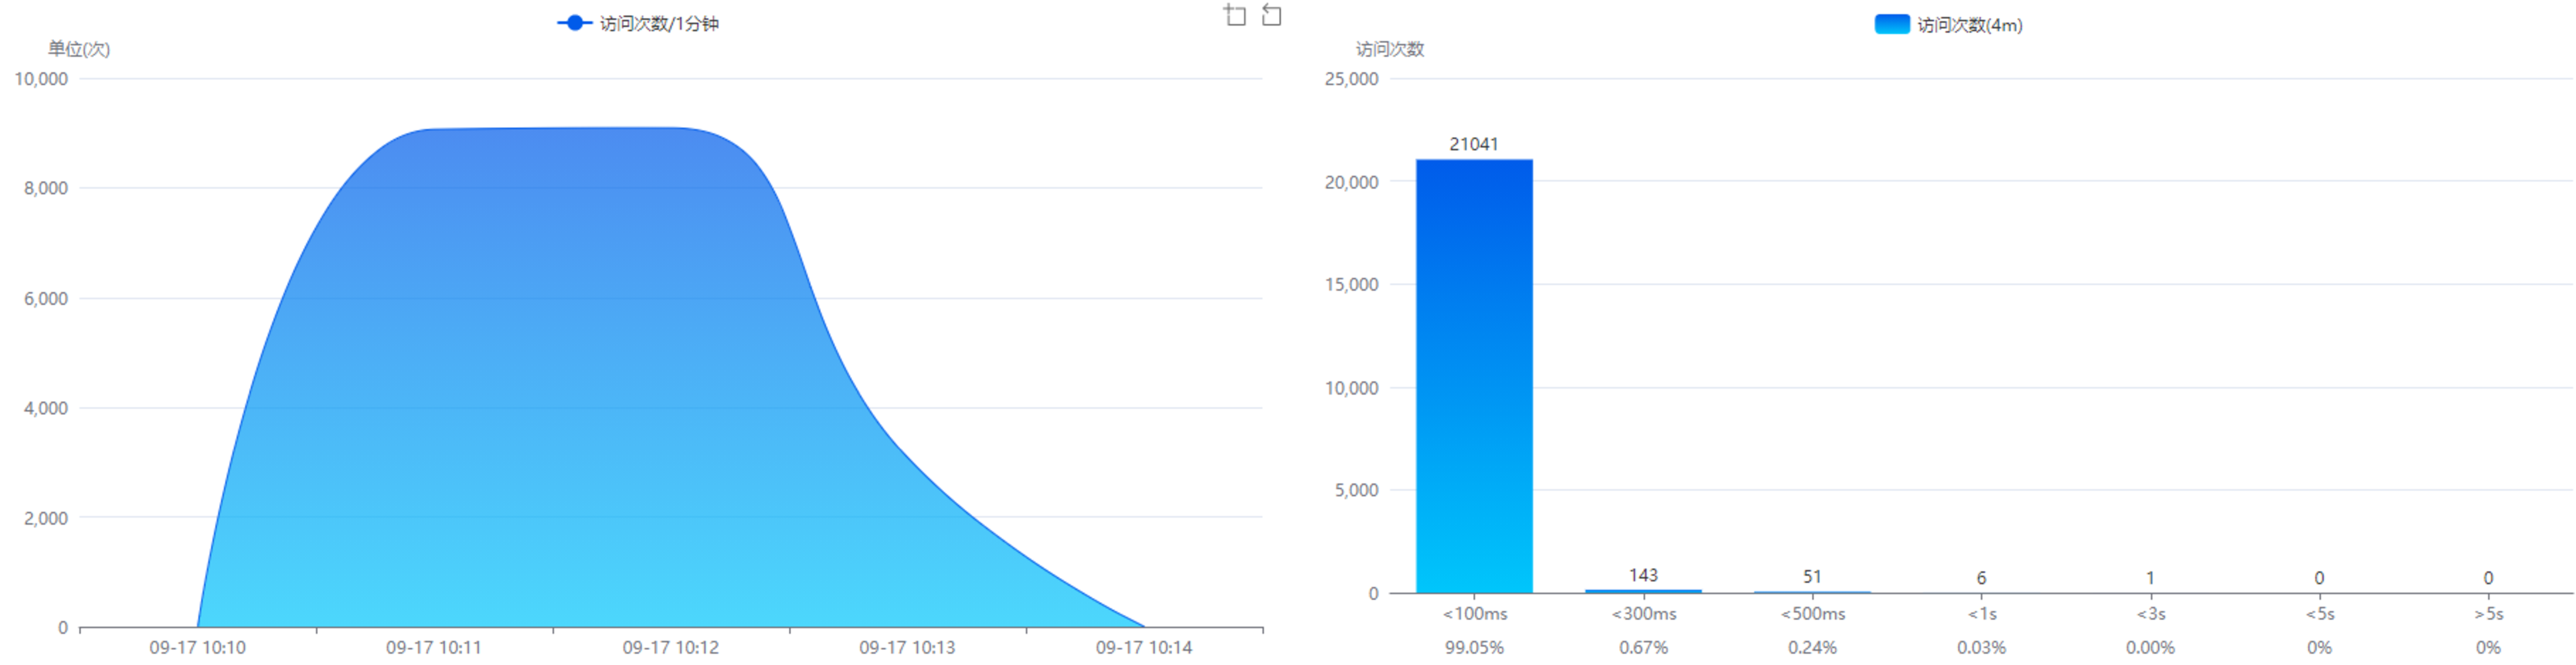
\includegraphics[width=1\textwidth]{压测.pdf}
    \caption{压力测试图}
    \label{fig:pressure}
\end{figure}


\subsection{易用性测试}

为了满足易用性测试,本系统在提供给用户使用时用户不需要关心数据库以
及前端页面的具体实现,用户只需根据自己的数据分析需求上传特定格式的文档即可,前端页面会自动渲染数据查询结果,以可视化的形式呈现数
据查询结果。因此发布的中文时间表达式信息抽取系统满足易用性的需求。

\subsection{兼容性测试}

为了满足兼容性测试,本系统的前端 Metis 页面分别在谷歌浏览器、Edge
浏览器、火狐浏览器、360 浏览器进行了测试,以上浏览器均能在 Metis 页面
上呈现功能测试中的各项数据,因此中文时间表达式信息抽取系统对以上各种
浏览器兼容。

\subsection{可维护性测试}

软件系统的可维护性可以用模块之间的耦合度、单元测试和集成测试的覆盖
率、代码规范等指标度量。本系统在开发过程中采用面向对象的设计方法,严格
遵循单一责任、低耦合高内聚等原则来进行系统模块的设计,减少模块与模块之
间的耦合度、增加模块内部的功能复用。系统在开发过程中也会在关键代码处添
加日志,当异常和错误情况发生时,开发人员能够快速通过日志进行问题解决。
综合以上分析,以太坊数据高速抽取和分析系统满足可维护性需求。

